%\documentclass[handout]{beamer}
\documentclass{beamer}
\usepackage[spanish]{babel}
\usepackage[ansinew]{inputenc}
\usepackage{amsmath}
\usepackage{enumerate}
\usepackage{exscale}
\usepackage{indentfirst}
\usepackage{latexsym}
\usepackage{proof}

\usepackage{tikz}
\usetikzlibrary{backgrounds,fit,arrows} 

%\usetheme{warsaw}

\newcommand{\lpobjective}[2]{\textsc{Objective:} #1 \[ #2 \]}
\newcommand{\lprestriction}[3]{\textsc{Subject to:} #1 \[ #2 \qquad #3 \]}
\newcommand{\lpineq}[2]{\[ #1 \qquad #2 \]}

\begin{document}

\title[A Branch \& Cut Algorithm for PCP]{A Branch \& Cut Algorithm for the Partitioned Graph Coloring Problem}
\author[Santiago Palladino, Isabel M�ndez-D�az, Paula Zabala]{Santiago Palladino, Isabel M�ndez-D�az, Paula Zabala \\ \{spalladino,imendez,pzabala\}@dc.uba.ar \\ \vskip 10pt \scriptsize{Facultad de Ciencias Exactas y Naturales \\ Universidad de Buenos Aires}}
\institute{Tesis de Licenciatura}
\date{June 2010}

\begin{frame}
\titlepage
\end{frame}

\setlength{\parskip}{10pt plus 1pt minus 1pt}

\section{Introducci\'on}
\subsection{Grafos}

\begin{frame}
\frametitle{Grafos}

\begin{definition}
Un grafo $G$ se define como un par $V,E$ donde $V$ es un conjunto de nodos, unidos por los ejes del conjunto $E$.
\end{definition}

\begin{figure}[h]
	\centering	
	\begin{tikzpicture} 
		[n/.style= {minimum size=3mm,thick,circle,draw=black}] 

		\node[n] (n0) at ( 0,0) {$v_0$}
		;

		\node[n] (n1) at ( 2,1) {$v_1$}
			edge [-]	(n0)
		;

		\node[n] (n2) at ( 2,3) {$v_2$}
			edge [-]	(n1)
		;
		
		\node[n] (n3) at ( 0,4) {$v_3$}
			edge [-]	(n1)
		;
		
		\node[n] (n4) at ( -2,3) {$v_4$}
			edge [-]	(n3)
			edge [-]	(n2)
		;
		
		\node[n] (n5) at ( -2,1) {$v_5$}
			edge [-]	(n2)
			edge [-]	(n4)
			edge [-]	(n0)
		;

	\end{tikzpicture} 
\end{figure}

\end{frame} 

\begin{frame}
\frametitle{Coloreo}

\begin{definition}
El problema de coloreo consiste en asignar un \textbf{color} a cada nodo de manera tal que dos nodos adyacentes tengan colores distintos.
\end{definition}

\begin{figure}[h]
	\centering	
	\begin{tikzpicture} 
		[n/.style= {minimum size=3mm,thick,circle,draw=black}] 

		\node[n] (n0) at ( 0,0) {$v_0$}
		;

		\node[n] (n1) at ( 2,1) {$v_1$}
			edge [-]	(n0)
		;

		\node[n] (n2) at ( 2,3) {$v_2$}
			edge [-]	(n1)
		;
		
		\node[n] (n3) at ( 0,4) {$v_3$}
			edge [-]	(n1)
		;
		
		\node[n] (n4) at ( -2,3) {$v_4$}
			edge [-]	(n3)
			edge [-]	(n2)
		;
		
		\node[n] (n5) at ( -2,1) {$v_5$}
			edge [-]	(n2)
			edge [-]	(n4)
			edge [-]	(n0)
		;

	\end{tikzpicture} 
\end{figure}

\end{frame}

\begin{frame}
\frametitle{Coloreo}

\begin{figure}[h]
	\centering
	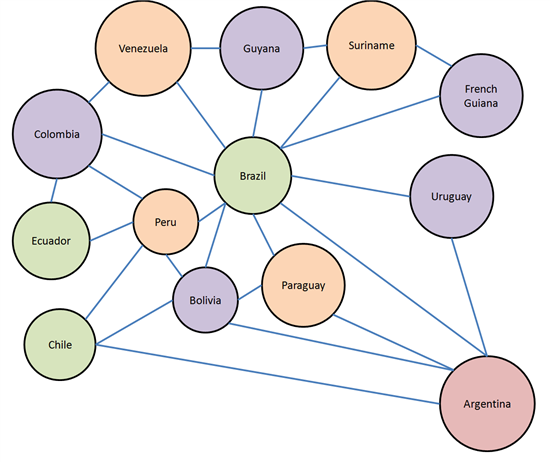
\includegraphics[scale=0.5]{../imgs/southamerica.png}
\end{figure}

\end{frame}


\begin{frame}
\frametitle{Grafos particionados}

\begin{definition}
Un grafo \textbf{particionado} es un grafo en el que el conjunto de nodos se encuentra dividido en particiones $P_0, \ldots,P_q$.
\end{definition}

\begin{figure}[h]
	\centering	
	\begin{tikzpicture} 
		[n/.style= {minimum size=3mm,thick,circle,draw=black}] 

		\node[n] (n0) at ( 0,0) {$v_0$}
		;

		\node[n] (n1) at ( 2,1) {$v_1$}
			edge [-]	(n0)
		;

		\node[n] (n2) at ( 2,3) {$v_2$}
			edge [-]	(n1)
		;
		
		\node[n] (n3) at ( 0,4) {$v_3$}
			edge [-]	(n1)
		;
		
		\node[n] (n4) at ( -2,3) {$v_4$}
			edge [-]	(n3)
			edge [-]	(n2)
		;
		
		\node[n] (n5) at ( -2,1) {$v_5$}
			edge [-]	(n2)
			edge [-]	(n4)
			edge [-]	(n0)
		;
		
		\begin{pgfonlayer}{background} 
			\node [fill=black!5,fit=(n0) (n1)] {}; 
			\node [fill=blue!5,fit=(n2) (n3)] {}; 
			\node [fill=green!5,fit=(n4) (n5)] {}; 
		\end{pgfonlayer}

	\end{tikzpicture} 
\end{figure}

\end{frame}

\begin{frame}
\frametitle{Coloreo particionado}

\begin{definition}
El problema de coloreo \textbf{particionado} consiste en, dado un grafo particionado, asignar un \textbf{color} a un solo nodo por particion, de manera tal que dos nodos adyacentes no usen colores iguales.
\end{definition}

\uncover<2->{
\begin{figure}[h]
	\centering
	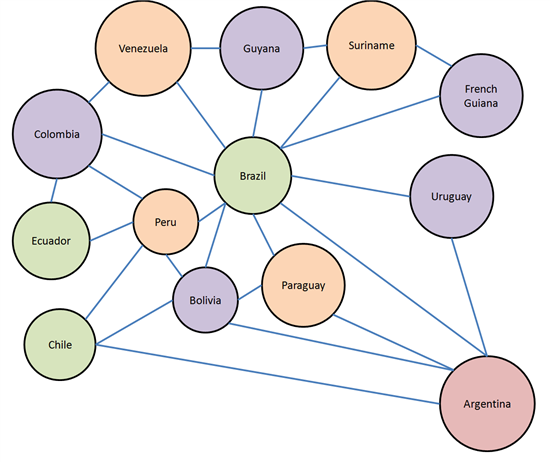
\includegraphics[scale=0.5]{../imgs/southamerica.png}
\end{figure}
}

\end{frame}

\begin{frame} 
\frametitle{Motivation}

Introduced as a means to solve the Routing and Wavelength Assignment (RWA) problem in Wavelength Division Multiplexed (WDM) optical networks.

Used to handle wavelength assignment conflicts between lightpaths sharing common fiber links, minimizing the number of wavelengths used, when all connection requirements are already known.

Other techniques to solve the RWA problem itself are out of the scope of this work.

\end{frame} 

\subsection{Related work}

\begin{frame} 
\frametitle{Related work}

\begin{description}[Noronha, Ribeiro; 2006]

\item[Li, Simha; 2000]{Greedy one step and two step heuristics}
\item[Noronha, Ribeiro; 2006]{Tabu search heuristic}
\item[Frota et al; 2009]{Branch and cut based on asymmetric representatives formulation}

\end{description}

\pause

We will propose an alternative integer programming formulation of the problem based on Mendez-Diaz and Zabala's model for standard coloring.

\end{frame} 

\section{Model}
\subsection{Model definition}

\begin{frame}
\frametitle{Model}

Every variable $x_{ij}$ is true if vertex $i$ is colored with color $j$. Variables $w_j$ are true if color $j$ is used in coloring the graph. 

\uncover<1->{
\lpobjective{Minimize sum of colors used}
{\min \sum_{j \in C} w_{j}}
}

\uncover<2->{
\lprestriction{Neighbours shall not have the same colour, and variable $w_j$ must be true if the color is to be used}
{x_{ij} + x_{kj} \leq w_j}{\forall j, \forall (i,k) \in E}
}
\uncover<3->{
\lprestriction{Every \only<3>{vertex}\alert<4>{\only<4>{partition}} has exactly one colour assigned}
{\uncover<4>{\sum _{x_i \in p}} \sum_{j \in C} x_{ij} = 1}{\forall i \in V \uncover<4>{, p \in P}}
}

\end{frame} 

\begin{frame}
\frametitle{Improving LP}

We also take symmetry breaking constraints from the original model and additional restrictions for eliminating fractional solutions.

\lprestriction{Color $j$ cannot be used unless color $j-1$ was used}
{w_{j} \leq w_{j-1}}{\forall j \neq 0 \in C}

\lprestriction{The label of a color used for a partition cannot exceed $\chi$}
{\sum_{j \in C} w_{j} \geq \sum_{x_i \in p} \sum_{j \in C} x_{ij}}{\forall p \in P}

\end{frame} 


\begin{frame}
\frametitle{Reworking adjacency constraints}

Adjacency constraints can be replaced by either of the following, which improve the relaxation's resolution.

\lprestriction{A node $i_0$ and all of its neighbours in a partition $p_0$ cannot share the same the color}
{\sum_{i \in p_0 \cap N(i_0)} x_{ij_0} + x_{i_0j_0} \leq w_{j_0}}{\forall i_0 \in V, j_0 \in C, p_0 \in P}


\lprestriction{A color $j_0$ may be used on a node $i_0$ or on at most $r$ of its neighbours, being $r$ the number of different partitions in $N(i_0)$}
{\sum_{i \in N(i_0)} x_{ij_0} + r x_{i_0j_0} \leq r w_{j_0}}{ \forall j_0 \in C, i_0 \in V}

\end{frame} 

\subsection{Valid inequalities}

\begin{frame}
\frametitle{Extended clique inequalities}

Let $K \subseteq V$ an \textit{extended clique} if for every pair $v,w \in K$, either $v$ and $w$ are adjacent or belong to the same partition.

We define the extended clique inequality as
\lpineq{\sum_{i \in K} x_{ij_0} \leq w_{j_0}}{\forall j_0 \in C}

We use a greedy heuristic to find maximal cliques in the graph which violate this inequality.

\end{frame} 

\begin{frame}
\frametitle{Block color inequalities}

Given the symmetry breaking constraints, a partition being coloured with any label greater or equal than $j_0$ is subject to $w_{j_0}$ being set.

This allows us to define the block color constraints as:
\lpineq{\sum_{i \in p_0}\sum_{j \geq j_0} x_{ij} \leq w_{j_0}}{\forall p_0 \in P, j_0 \in C}

All these constraints are simply handled by brute force.

\end{frame} 

\begin{frame}
\frametitle{Component independent set inequalities}

Let $I \subseteq V$ be a \textit{component independent set} if for every pair $v,w \in I$, $v$ and $w$ are not adjacent and belong to different partitions.

This allows us to reuse the independent set inequality from the standard coloring problem.
\lpineq{\sum _{i \in I} x_{ij_0} \leq \alpha(I) w_{j_0}}{\forall j_0 \in C}

\pause

Which can be strengthened considering symmetry breaking.
\lpineq{\sum _{i \in I} x_{ij_0} + \sum ^n _{j = n - \alpha(I) + 1} \sum _{i \in V} x_{ij} \leq \alpha(I) w_{j_0} + w_{n - \alpha(I) + 1}}
{\forall j_0 \leq n - \alpha(G)}

\end{frame}

\begin{frame}
\frametitle{Hole and path inequalities}

Component independent set inequalities can be specialized as component hole and component path inequalities, using $\lfloor |H|/2 \rfloor$ and $\lceil |P|/2 \rceil$ respectively as their cardinals.

We use a greedy heuristic constructing a path from each node for each colour. The criteria for choosing a node is based on its corresponding $x_{ij}$ value and whether it has been previously visited or not.

\end{frame}

\begin{frame}
\frametitle{G' independent set inequalities}

Given a partitioned graph $G=(V,E,P)$, we define the graph $G'=(V',E')$, with $V' = P$ and $E'$ such that $p_1,p_2 \in V'$ are adjacent iif every node in partition $p_1$ in $G$ is adjacent to every node in partition $p_2$ in $G$. More formally:
\[
E' = \{(p_1,p_2) : p_1,p_2 \in V' \wedge \forall v \in p_1 \forall w \in p_2 : (v,w) \in E \}
\]

\pause

This grants another way to reuse independent set inequalities from the standard coloring problem; let $I'$ be an independent set in $G'$, then:

\lpineq{\sum_{p \in I'} \sum_{i \in p} x_{ij_0} \leq \alpha(I') w_{j_0}}{\forall j_0 \in C}

\end{frame}

\section{Branch \& Cut}

\begin{frame}
\frametitle{Branch and Cut}

Using the model previously defined along with the valid inequalities implemented as cutting planes, we implemented a branch and cut algorithm to tackle this problem, adding initial and primal heuristics and specific branching strategies.

\end{frame} 

\subsection{Preprocessing}

\begin{frame}
\frametitle{Preprocessing steps}

The following steps are taken to preprocess the graph:
\begin{itemize}

\item{All edges within a partition are removed}
\item{All partitions with an isolated vertex are removed}
\item{All nodes $v$ such that $N(u) \subseteq N(v)$ for a node $u$ in the same partition are removed}

\end{itemize}

\end{frame} 


\subsection{Cuts}

\begin{frame}
\frametitle{Cutting planes}

We implemented the inequalities in the previous section as cutting planes, tested initially in a Cut and Branch algorithm, and then added to a Branch and Cut structure.

Cuts are applied aggressively on the root of the branching tree, and with fewer iterations on the rest of the tree until a certain depth, in order to keep relaxations easy to solve.

\end{frame}

\begin{frame}
\frametitle{Cutting planes}

The cuts with the best performance were Extended Clique and Block Color, and are therefore the most aggressively applied. 

Component independent set and $G'$ independent set cuts are applied only if a minimum number of the previous cuts is not found.

\end{frame}

\subsection{DSatur}
\begin{frame}
\frametitle{DSatur}

DSatur is an exact method for finding an optimal coloring for a graph by implicitly enumerating all possible colourings.

It is a sequential algorithm in which nodes are chosen based on the \textit{degree of saturation}: the number of different colours used for its neighbours in the current solution. 

Harder nodes (higher 
degree of saturation) are chosen first.

\end{frame} 

\begin{frame}
\frametitle{Extending DSatur}

Classic DSatur is used for standard colouring. We propose two extensions for partitioned colouring:

\begin{itemize}

\item{\textit{Easiest node:} We first select the easiest node (lowest degree of saturation) to be coloured in each partition, and then we apply standard criteria to pick the hardest one from that set.}

\item{\textit{Hardest partition:} We first pick the hardest partition to be coloured according to its degree of saturation, size and uncoloured nodes; and then we pick the easiest node (lowest degree) from that partition.}

\end{itemize}

\end{frame} 

\begin{frame}
\frametitle{Heuristics}

Although DSatur is an exact algorithm, it quickly generates good enough solutions, therefore being a good heuristic by bounding the number of iterations or time.

DSatur proved to be an excellent initial heuristic, sometimes actually arriving to the optimal solution by itself.

We also adapted it to serve as a primal heuristic by fixing all nodes with a high enough value in the relaxation and executing DSatur on the remaining ones.

\end{frame} 

\subsection{Branching}
\begin{frame}
\frametitle{Branching priorities}

We implemented a static branching strategy for $x_{ij}$ variables prioritizing on:

\begin{itemize}
\item{The higher the number of partitions adjacent to node $i$}
\item{The smaller the size of the partition where node $i$ is}
\item{The higher the colour label $j$}
\end{itemize}

\end{frame}

\begin{frame}
\frametitle{DSatur branching}

A second branching strategy implemened was picking the nodes with the highest degree of saturation in the current solution.

The previous strategy was used as a tie-breaker for nodes with equal degree, picking a single node $i_0$.

The chosen $x_{ij}$ variable for branching was the one with the highest value among all $x_{i_0j}$.

\end{frame}


\begin{frame}
\frametitle{Pruning}

When the number of $x_{ij}$ variables fixed to $1$ during the branching process is high enough, we stop the branch and cut algorithm in that node, pruning the subtree.

The exact solution corresponding to that node is found using DSatur as an exact algorithm, enumerating all possible colourings of the remaining partitions.

\end{frame}

\section{Results}
\subsection{Implementation}

\begin{frame}
\frametitle{Implementation}

The previous algorithm was implemented in Java $1.6$ on top of Cplex $12.1$ and executed on a $2.80$ GHz core with $4$ Gb RAM. 

We implemented both a Cut and Branch and a Branch and Cut algorithm to test the effectiveness of the strategies devised.

Note that work is still in progress and the implementation, much less its parametrization, is not final.

\end{frame}

\begin{frame}
\frametitle{Test Suites}

We built two test suites with random generated graphs:
\begin{itemize}
\item Fixed density of $50\%$, nodes from $60$ to $90$
\item Fixed node count of $80$, density from $20\%$ to $80\%$
\end{itemize}

Partition size for both suites was fixed to $2$. 

Each set was run for 30 minutes and the solution gap and node count in the branch tree is reported for both Branch and Cut and Cut and Branch.

\end{frame} 

\subsection{Preliminary Results}

\begin{frame}
\frametitle{Fixed node count}

\begin{center}
\begin{tabular}{|c|cc|cc|}
\hline
\multicolumn{1}{|c|}{Graph} & \multicolumn{2}{|c|}{Branch \& Cut} & \multicolumn{2}{|c|}{Cut \& Branch}
\\
\hline
density & nodes & gap & nodes & gap 
\\
\hline
0.2 & 485 &    0.00 & 2536 &    0.00
\\
0.4 & 1362 & 0.30 & 31209 & 0.48
\\
0.6 & 377 & 0.41 & 7329 & 0.50
\\
0.8 & 225 & 0.46 & 5135 & 0.51
\\
\hline 
\end{tabular}
\end{center} 
 
\end{frame} 

\begin{frame}
\frametitle{Fixed density}

\begin{center}
\begin{tabular}{|c|cc|cc|}
\hline
\multicolumn{1}{|c|}{Graph} & \multicolumn{2}{|c|}{Branch \& Cut} & \multicolumn{2}{|c|}{Cut \& Branch}
\\
\hline
nodes & nodes & gap & nodes & gap 
\\
\hline
60 & 3039 &    0.00 & 121779 & 0.22
\\
70 & 1856 & 0.29 & 54437 & 0.38
\\
80 & 1077 & 0.31 & 25909 & 0.40
\\
90 & 244 & 0.45 & 5817 & 0.51
\\
100 & 337 & 0.54 & 13267 & 0.58
\\
\hline 
\end{tabular}
\end{center}
  
\end{frame} 

\subsection{Future work}

\begin{frame}
\frametitle{Future work}

\begin{itemize}

\item{Theoretical analysis of the polytope}

\item{Implement more families of cutting planes}

\item{Optimize primal and separation heuristics}

\item{Build a larger and more comprehensive test suite}

\item{Determine optimal parametrizations for different graphs}

\item{Check performance of full branch and cut on larger instances}

\end{itemize}

\end{frame}

\begin{frame}

\begin{center}
\LARGE{Questions...?}
\end{center}

\end{frame}

\end{document}


